%===================================== CHAP 3 =================================

\chapter{Methods and implementation}\label{chpt:methods}

\textbf{Notes}

Where should the focus be? \textit{pseudopattern generation and memory consolidation}

HPC module - high-quality pattern extraction, STM with sufficiently high degradation of old memories to avoid dilution and spurios memories

neocortical module - pattern acquisition, acquisition of functional mapping

Analyzation - see notes.
\\

Choices I have made in the implementation that remains unclear in the paper.

Enforce sparsity through weight updates corresponding only to the winners of kWTA.
Alternatively: Through initializing synapses only for a given (local) percentage of neurons.

(Could normalize the weights vector)
Although possibly not entirely biologically plausible, normalization increases the ability of separation, because it maps vectors to points on a hypersphere, enhancing the hyperplane separability. (p. 60)
Normalization should occur in the model. Oja's rule is explicit weight normalization. The other which is used is implicit. (p. 72).

negative weights will necessarily allow for more categorization, and possibly avoiding learning the mean feature vector. However, it reduces perfect recall rates (p. 74) - this may affect especially heteroassociation.

\section{Concepts}
\subsection{Information processing capabilities}

Lateral inhibition

kWTA - separation, segmentation, etc.

Biologically, original experiment from \citep{Hattori2014} from [other paper] .. testing STM, several aspects.

\section{Theano - a Python library as framework}

Theano is a Python library for building high-performance mathematical tools \citep{Bergstra2010}. It lets you write library-specific code which will be analyzed, optimized, and compiled to C or CUDA, enabling execution of efficient bytecode. Furthermore, Theano lets you symbolically define an algorithm in a high-level programming environment. For those familiar with Mathematica, symbolic definition in Theano is fairly similar. In this thesis Theano is used for model implementation, the experiments being outlined in chapter \ref{chpt:experiments}.

\subsection{A Brief Overview}

Theano is tightly integrated with NumPy, another Python package for scientific computation. Moreover, Theano supports parsing of several NumPy objects into objects which Theano will be able to later use efficiently after its optimization process. Please consult LISA lab's webpage \citep{LISA-lab2015a} for a complete documentation of the framework.
Theano operates on symbolic constructs, called tensors; general mathematical constructs. So in order to define a function, you would write the actual mathematical expression, for instance:

\begin{verbatim}
import theano.tensor as T
import theano

A = T.fmatrix('A')

y = A ** 2

f = theano.function([A], y)
\end{verbatim}

Calling the library function theano.function analyses the symbolic expression, and constructs executable C or CUDA code from it. To further demonstrate the flexibility of using symbolic expressions, an example of calculating numbers of the Fibonacci sequence is included below (imports as above being presumed):

\begin{verbatim}
def fib_acc(old, older):
    return old + older

fib_expr, updates = theano.scan(
    fn=fib_acc,
    sequences=None,
    outputs_info=[dict(initial=np.int32([0, 1]), 
    taps=[-1, -2])], n_steps=n)

f_fib_scan = theano.function([n], fib_expr)
\end{verbatim}

Note that the recursive definition is captured by theano.function. When theano.function is called, the first parameter it takes is the input parameters for the function that is to be calculated.
Preceding the input parameters are the output parameters which are the expressions to be calculated. It is further possible to specify among other expressions the \textit{updates} for new shared variables. By providing 'updates' = [variables] to the function, the variables will be kept in the shared variable \textit{updates}. Furthermore, \textit{givens} may be supplied for substitutions in the computation graph (i.e. if a function should be substituted with a given value such as a constant).
In order to loop over a function, the \textit{scan}-function of the Theano-library may be used. Scan performs an optimized looping over a symbolic graph, letting the user define parameters for optimizing the iteration. For instance it lets the user tell Theano that some variables do not need to be stored, thus the compiler re-uses a register for the variable as it is updated, potentially speeding up the loop. Scan may further be used to dramatically speed up matrix-vector multiplication.
Note that Theano may take a normal Python function-object as an input function to the scan-operator. Standard Python code of the f\_fib\_scan loop would be to call fib\_acc(...) in a for-loop. Furthermore, scan lets the programmer explicitly define recursive relationships for output expressions that are to be computed using the taps-variable, which here states that the two former variables are to be kept in memory. Note that this requires one to define the initial values of the parameters. Theano supports both exclusive and inclusive scan (appending one element at a time for input to the binary function as opposed to supplying all combinations of the input).

When defining symbolic expressions such as functions using Theano, Theano constructs a graph of the provided symbolic expressions, see figure \ref{fig:theano_graph_demo}. This allows for differentiation and manipulation through a syntactic and semantic analysis of the resulting expression graph, optimizing the graph for expression evaluation and graph traversal before code generation. The compiler may then generate optimized code, compiling it according to the provided environmental parameters. This leads to highly efficient C or CUDA executable code.
Note, however, that as the library provides a high-level abstraction for generation of efficient C or CUDA-code, this renders debugging somewhat harder. More specifically, the executable code will be further processed from that in Python and Theano. This means that the programmer may need to predict more about how the code will be compiled, making it highly recommendable or necessary to have some previous knowledge within C and/or how the Python-library's compilation process works. A remedy for this is howeevr that Theano supports profiling, providing the programmer with information about what data structures the variables are compiled to, as well information about as their usage. Furthermore, if compiling to a GPU, Theano may output warnings whenever an operation is performed on the CPU.

\begin{figure}
\centering
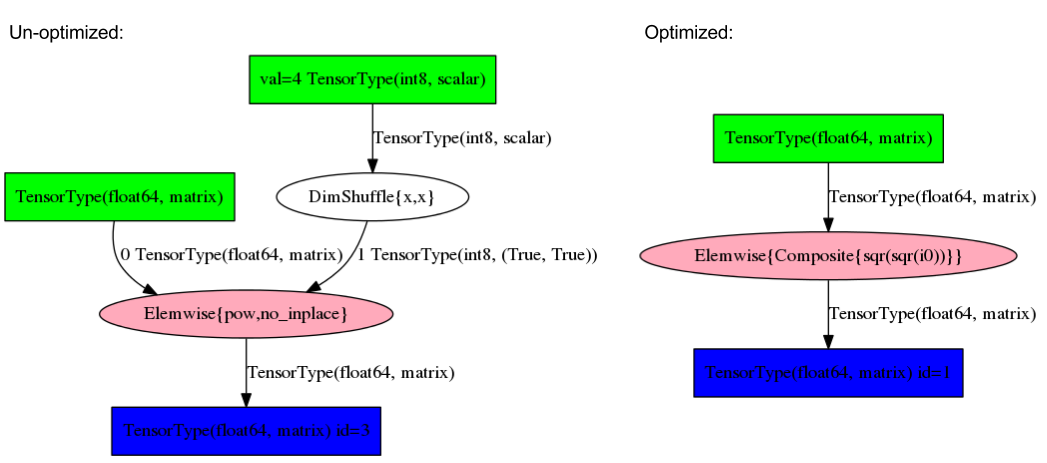
\includegraphics[width=10cm]{fig/unopt_opt_theano_graph}
\caption{Graph manipulation of tensors in Theano during the optimization and compilation process of the expression $y = A^2$ from the first code example of this section.}
\label{fig:theano_graph_demo}
\end{figure}

\subsection{Setup}

In order to use Theano, certain dependencies need to be setup. These are fairly straightforward when it comes to compiling to C-code for CPU-execution. In a preliminary study for this thesis, I setup Theano for use with a GPU on a system with an NVIDIA card, using Ubuntu 14.04 LTS. I consulted the guide found on \citep{LISA-lab2015b} to obtain installation instructions for doing so. In doing so I noticed that the complex logics of the dual-network memory model required it to be synchronized, thus requiring transferring control to the CPU and interpreter, including memory transfer from the GPU to the CPU. Therefore, running the model on the GPU is not regarded as providing run-time performance gains, and the model targets the CPU (particularly the HPC-module, which may only be executed on the CPU).

\section{Algorithmic outline}

Class HPC encapsulating shared variables and methods specific for the STM-network.

Example of weight matrix and associated theano functions.

System layout figure

learn-wrapper, the main method; excerpt

neocortical network; simple, efficient

DNMM spanning both networks.

experiments suite - two as outlined by \citep{Hattori2014}, originally retrieved from ... as outlined above
enabling several trials automatically.
cPickle
PIL
Tools \^
file-handling

test suite to ensure partial model correctness / improve quality and automate development


\section{Parametrization and model decisions}

hpc = HPC([io\_dim, 240, 1600, 480, io\_dim], \\
          0.67, 0.25, 0.04,  \# connection rates: (in\_ec, ec\_dg, dg\_ca3) \\
          0.10, 0.01, 0.04,  \# firing rates: (ec, dg, ca3) \\
          0.7, 100.0, 0.1, turnover\_rate,  \# gamma, epsilon, nu, turnover rate \\
          0.10, 0.95, 0.8, 2.0, weighting\_dg)  \# k\_m, k\_r, a\_i, alpha. alpha is 2 in 4.1
          
Implementation of nu- and zeta-functions in CA3. Thresholding after equation calculations

One recall iteration in CA3 for each total recall iteration.

Turnover between every training set iteration (?). Needs to include empirical data on decision making. Move to preliminary experimentation in chpt. 4?

Heavier weighting DG. Based on paper \citep{Norman2003}. Empirical results. Chpt. 4. Figures. Nice.